In the evaluation section for DRIVE system, we briefly mentioned the custom 
simulator that
we built to perform the quantitative analysis of IODEDUP system's efficiency,
as well as to evaluate the performance of the DRIVE system in comparison
with the Vanilla and IODEDUP systems. In this Appendix, we describe the
design and implementation of the simulator, called \texttt{SimReplay},
in more detail.

The main requirement from the simulator is that it capture the functionality of
the Vanilla, IODEDUP and DRIVE systems and demonstrate the effect of
each of these I/O access mechanisms on the cache efficiency and read
access performance. 
We have built the simulator to be modular so that it could be used to
develop and test new I/O deduplicate \& redirection strategies as well.

\begin{figure}[h]
    \centering
    %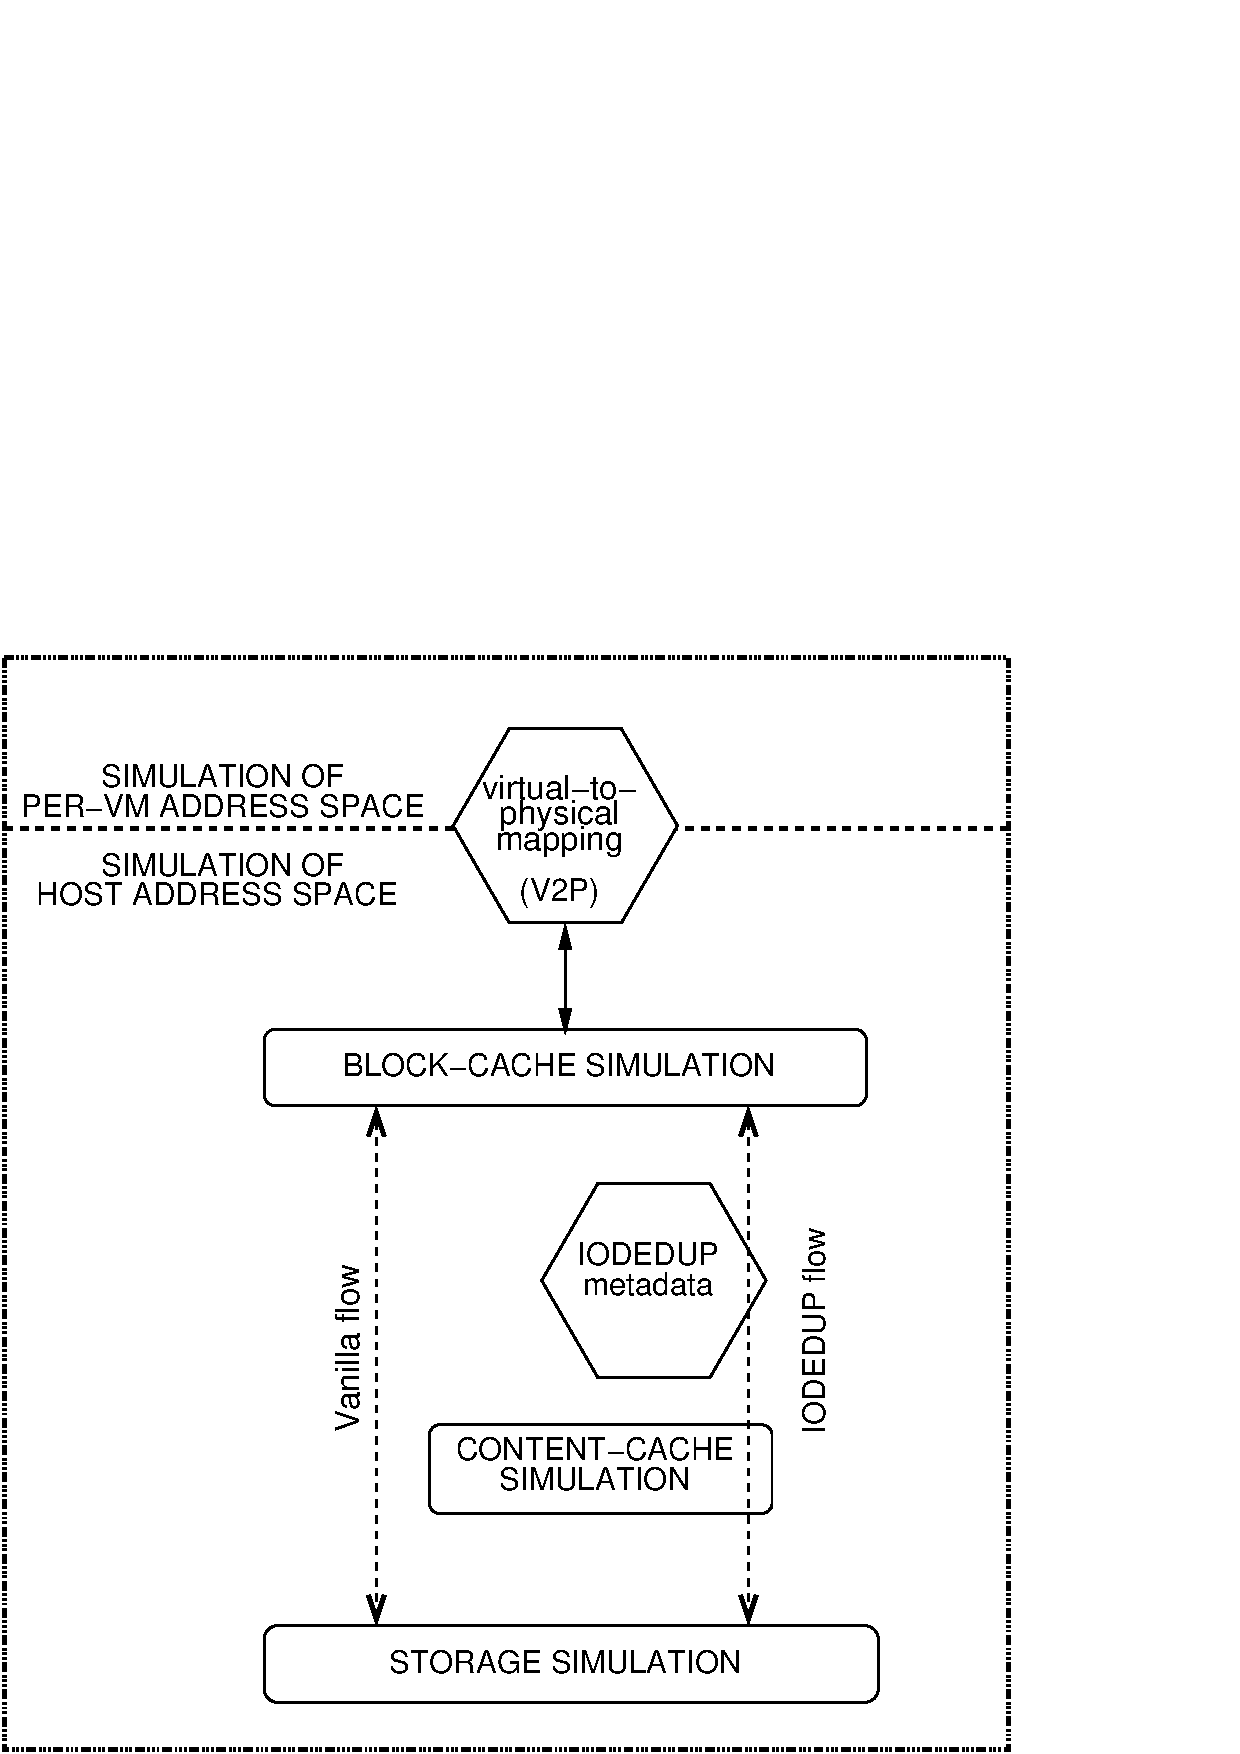
\includegraphics[scale=0.6]{simreplaychap-figures/simreplay-requirements.pdf}
    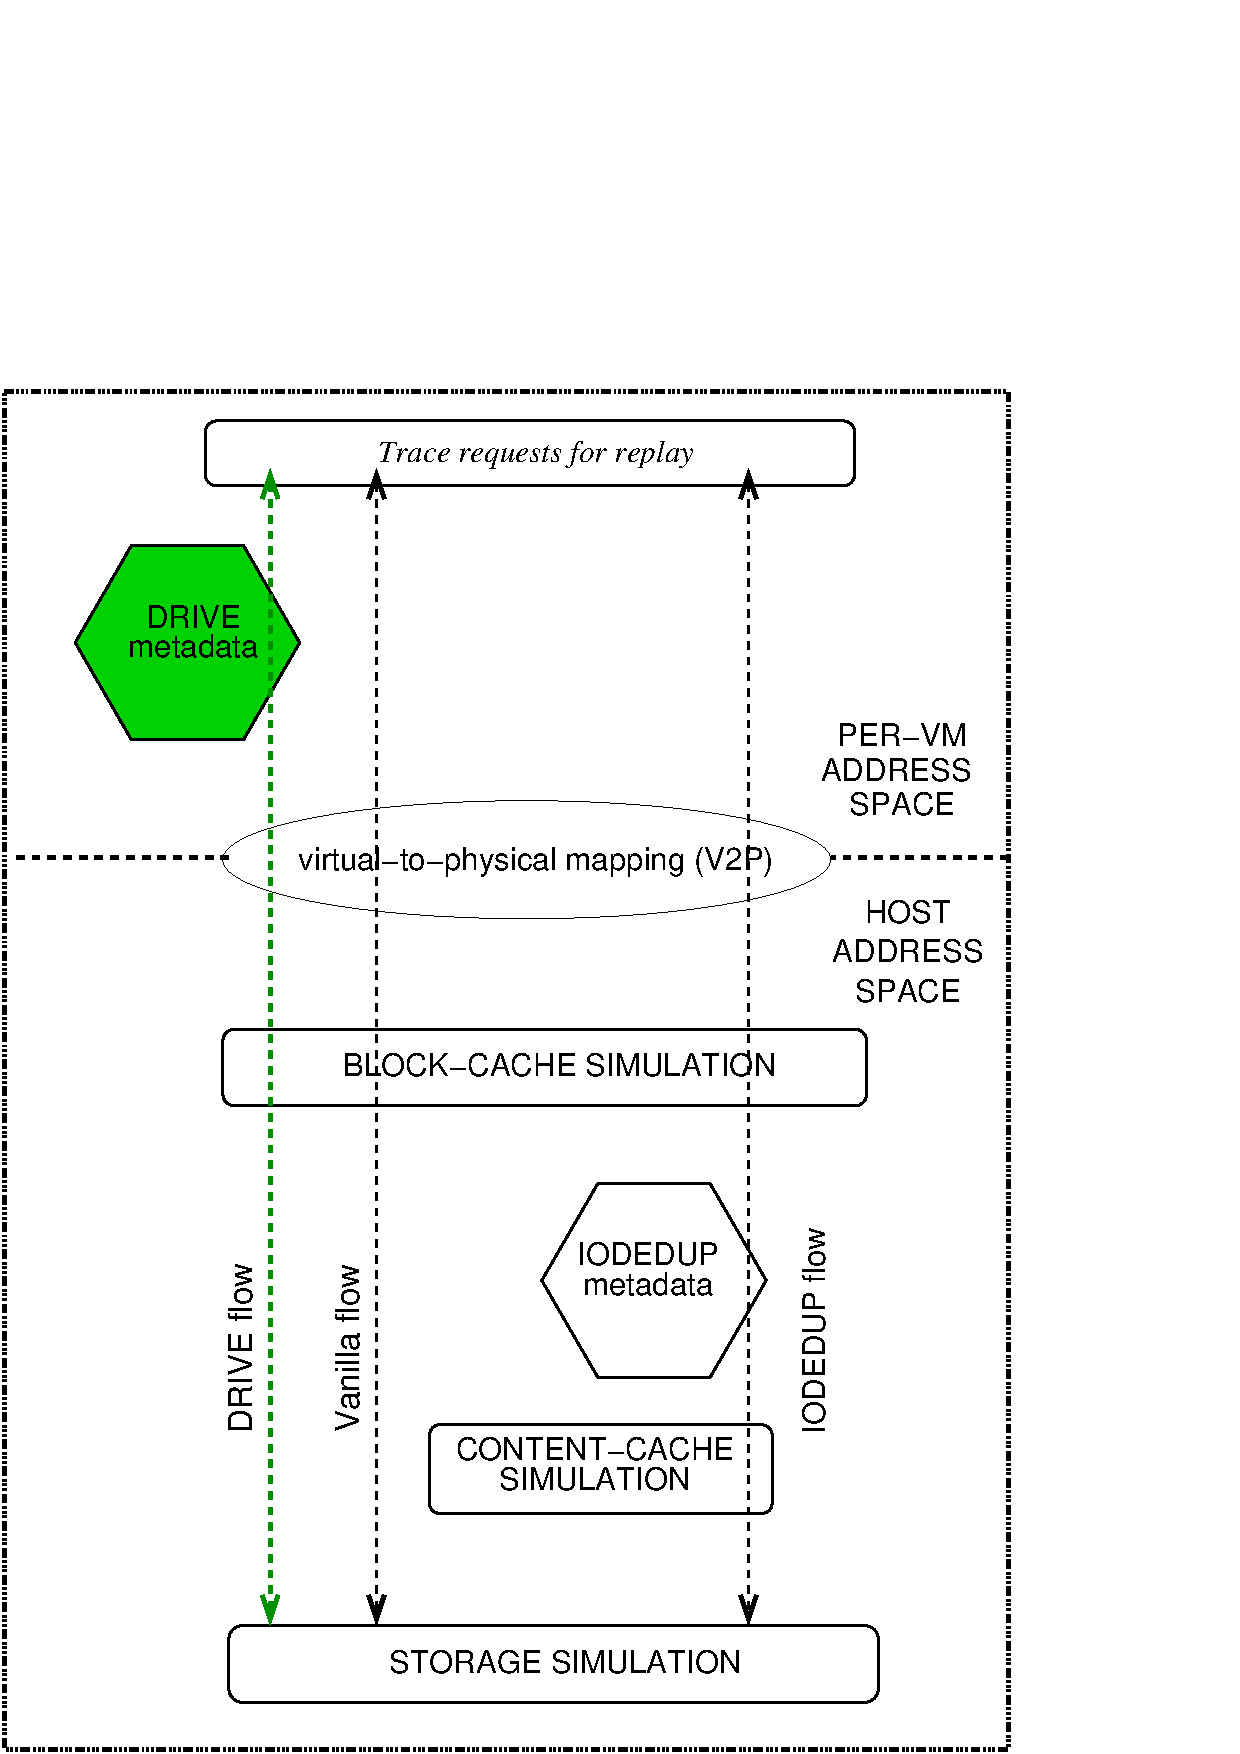
\includegraphics[scale=0.55]{simreplaychap-figures/simreplay-drive-extension.pdf}
    \caption{High-level functioning and requirements: \textit{The simulator should perform 
			simulation of I/O replay by simulation of a per-VM address space 
			and a host address space. It should accept an input 
			virtual-to-physical (V2P) mapping for these two address spaces. 
			It should also simulate a block-cache as well as storage for
			Vanilla, IODEDUP and DRIVE invocations, 
			and a content-cache especially for IODEDUP invocation.}}
    \label{fig:simreplay-requirements}
\end{figure}

\section{High-level functioning and requirements}
The simulator basically accepts virtual disk requests from multiple VMs
hosted on a single physical machine, and simulates its I/O execution
on the physical machine. The I/O execution in the standard case is referred 
to as Vanilla, while the augmented execution scenario presented
in \cite{iodedup} is referred to as IODEDUP. A third execution 
scenario in this simulator is our system called DRIVE.
Since the simulation is of virtual disk requests sent by VMs, an input 
mapping needs to specify which virtual disk block of a VM maps to which
corresponding physical disk block on the physical host's storage.
Two main components of the simulator are the simulation of two 
caches on the physical host: 
(i)~a block-based (LRU) cache and (ii)~a content-based (ARC) cache, both
of configurable sizes and using write-through policy. 
Additionally, the physical host's disk or storage also needs to be simulated. 

Fig. \ref{fig:simreplay-requirements} depicts the functioning 
of the custom simulator.
As shown, a virtual disk request is mapped from the virtual address space to
the host physical address space, and then looked-up in host's block-cache.
In case of Vanilla flow, the requests flow from the block-cache straight
to the host storage. On the other hand, in case of IODEDUP flow, 
metadata is looked up for every request that is not satisfied by the
block-cache, and content is searched in the content-cache, before hitting
the host storage. In case of DRIVE flow, the requests are redirected
within the virtual machine address space itself, so that the flow path
within the physical machine address space remains unchanged (i.e., same
as Vanilla path on physical machine).

The input to the simulator is a single trace file which contains multiple
disk read/write requests. 
Each request in the trace should contain information regarding
(i)~whether it is a read or write request,
(ii)~block number to be read or written,
(iii)~data to be read or written, and its size.
The output from the simulator involves the collection of metrics like
number of cache-hits and cache-misses incurred over the execution of
all requests in the trace file.
Next, we present the high-level and low-level design descriptions 
for the custom simulator. Finally, we present details regarding the
implemented input options and demonstrate the usage of the simulator.

\section{High-level design}
\label{sec:simreplaychap-design}

\begin{figure}[t]
    \centering
    \includegraphics[scale=0.6]{simreplaychap-figures/simreplay-interaction.pdf}
%    \vspace{-0.1in}
    \caption{Modules of the simulator: \textit{The IODEDUP execution logic 
		needs to maintain deduplication metadata, and hence requires a 
		content finger-printing module as well (eg. MD5, SHA). Additionally,
		modules to measure number of cache-hits \& misses, as well as
		to measure content deduplication ratio achieved in total cache space,
		are shown.}}
    \label{fig:simreplay-interaction}
%    \vspace{-0.2in}
\end{figure}

Fig. \ref{fig:simreplay-interaction} depicts the different modules 
of the custom simulator, and the interaction among them. For each of
the above modules, a brief description is given next.

%\subsubsection{Mapping from virtual disk space to physical disk space}
\subsection{Virtual-to-physical address mapping}
\label{sec:simreplaychap-v2p}
The input Virtual-to-physical (V2P) address mapping
indicates the range of physical blocks (i.e. blocks on host storage)
that map to the address space of each VM (i.e. blocks of virtual disk)
for simulation. This input applies to all the three invocations
of the simulator\textemdash{}Vanilla, IODEDUP and DRIVE.

%\lstset{language=bash,
%	caption={Output of command \texttt{df -h} on test machine.},
%	label=lst:df-h
%}
%\begin{snippet}
%root@PM5:~# df -h
%Filesystem            Size  Used Avail Use% Mounted on
%/dev/sda1             230G  208G  9.9G  96% /
%none                  3.0G  240K  3.0G   1% /dev
%none                  3.0G     0  3.0G   0% /dev/shm
%none                  3.0G  132K  3.0G   1% /var/run
%none                  3.0G     0  3.0G   0% /var/lock
%none                  3.0G     0  3.0G   0% /lib/init/rw
%/dev/sdb1             917G  388G  483G  45% /NFSDIR3
%\end{snippet}

\paragraph{Assumptions.} The assumptions made regarding the V2P map are
the following:
(i)~All blocks belonging to a single virtual disk are contiguous blocks on
the host storage, and
(ii)~Block requests are aligned at 4KB (i.e. 8 sectors) boundaries.
%Next, we explain the significance and implications of each of these
%assumptions.
The first assumption is a simplifying assumption
for ease of implementation of the simulator, and discarding this assumption
should not have any significant impact on the results presented in this thesis.
The second assumption holds true if the 
starting sector number of the host storage partition is a multiple of eight (8),
which should be the case in efficiently configured storage systems.
However, if this is not the case, 
the performance of the system/applications would be affected in general~\cite{virt-alignment-scan},
and an administrative fix during configuration is recommended to avoid
such inefficiency~\cite{netapp-alignment, oracle-alignment}.

\lstset{language=bash,
	caption={Output of command \texttt{fdisk -l} on test machine.},
	label=lst:fdisk-l
}
\begin{snippet}
root@PM5:~# fdisk -l

Disk /dev/sda: 500.1 GB, 500107862016 bytes
255 heads, 63 sectors/track, 60801 cylinders
Units = cylinders of 16065 * 512 = 8225280 bytes
Sector size (logical/physical): 512 bytes / 512 bytes
I/O size (minimum/optimal): 512 bytes / 512 bytes
Disk identifier: 0x0003741c

   Device Boot      Start         End      Blocks   Id  System
/dev/sda1   *           1       30395   244140032   83  Linux
/dev/sda2           60055       60802     5995521    5  Extended
/dev/sda3           30395       60055   238247936   83  Linux
/dev/sda5           60055       60802     5995520   82  Linux swap

Partition table entries are not in disk order

Disk /dev/sdb: 1000.2 GB, 1000204886016 bytes
255 heads, 63 sectors/track, 121601 cylinders
Units = cylinders of 16065 * 512 = 8225280 bytes
Sector size (logical/physical): 512 bytes / 4096 bytes
I/O size (minimum/optimal): 4096 bytes / 4096 bytes
Disk identifier: 0x000aff6c

   Device Boot      Start         End      Blocks   Id  System
/dev/sdb1               1      121601   976760001   83  Linux
Partition 1 does not start on physical sector boundary.
\end{snippet}

\paragraph{Example Partition Layout.} 
The list of partitions and the starting sector of all 
partitions on a linux host can be viewed using the commands 
\texttt{df -h} and \texttt{fdisk -l}, respectively. 
The sample output from one of our test machines is shown below in 
%Listings \ref{lst:df-h} and \ref{lst:fdisk-l}.
Listing \ref{lst:fdisk-l}.
%The Listing \ref{lst:df-h} shows that there are two hard-disks (sda \& sdb)
%mounted on the test machine, of which sda is the booting partition, and
The listing \ref{lst:fdisk-l} shows the ``Start'' sector number, 
``End'' sector number and the total number of ``Blocks'' for each partition,
for each hard-disk present.
% (The extra entries sda2, sda3, sda5 in 
%output of \texttt{fdisk -l} indicate swap partitions as well as 
%partitions installed with other operating systems, and hence do not seem to
%show up in output of \texttt{df -h}).
It can be seen that none of the ``Start'' sector numbers are aligned at
4K boundaries. This is the case because the system was installed for
test usage only, and not for performance-optimized usage. 
However, in
production servers and cloud usage, it is expected that the disk would
be formatted and partitioned correctly for optimized performance.

\paragraph{Effect of non-aligned block requests.}
The block-cache operates at 4KB page granularity, and if a block write
request is received for a \textit{whole} 4KB block, the block is directly 
written to cache without needing to first fetch it from disk. However,
if the block write request is only for a \textit{partial} block, the 
block needs to be first fetched from disk, and then the partial write
is performed to it so that when the resulting buffer is flushed to disk,
the unwritten portion of the block remains unchanged.
Given the above, if a block being written to the block-cache is not 
aligned (i.e. one block write request results in two partial block writes), 
two blocks would need to be first fetched from disk into cache, and 
then both would need to be partially over-written. 
Similarly, a single block read request would also necessitate the read of two
blocks from disk.
In our simulation, we have done away with such complexities by assuming 
that all block requests are block-aligned. As specified earlier, this can be
achieved in a straight-forward manner by correct configuration of
the physical storage.

%\begin{figure}[t]
%    \centering
%    \includegraphics[scale=0.6]{simreplaychap-figures/simreplay-v2pexample.pdf}
%%    \vspace{-0.1in}
%    \caption{Example V2P map input file. Each 3-tuple specifies the range
%			of block addresses for a single VM. There should be no
%			overlap between the ranges specified for different VMs.}
%    \label{fig:simreplay-v2pexample}
%%    \vspace{-0.2in}
%\end{figure}

\paragraph{Example V2P map input.}
Since all blocks of a single VM are assumed to be in a contiguous chunk on
host storage, the representation of the resulting V2P map is simplified.
Suppose there are three VMs, each having a virtual disk of 1000 blocks each.
Thus, on the host storage, these three VMs can be assumed to be laid out
such that the first VM's (VM1) blocks map to physical blocks 0-999, 
the second VM's (VM2) blocks map to physical blocks 1000-1999, and the
third VM's (VM3) blocks map to physical blocks 2000-2999. 
In our simulator, the above information is input in terms 
of a 3-tuple per VM like 
$<$\textit{vmname}, \textit{capacity}, \textit{base-address}$>$.
In the 3-tuple representation, \textit{capacity} refers to the number of
blocks in the VM (i.e., 1000 in above example) and \textit{base-address}
refers to the starting address in the host storage (0, 1000, 2000 
for each VM respectively, in above example). 
%Fig. \ref{fig:simreploay-v2pexample} shows the same example pictorially. 
Note that the \textit{base-address} can be any value, provided that the
range of addresses for none of the VMs overlap with each other.

\subsection{Block-cache \& Content-cache simulation}
The block-cache is simulated with the Least Recently Used (LRU) policy
for cache eviction as well as the write-through policy for handling
block writes. The size of the block-cache is configured by default 
to be 1GB, and can be tuned according to requirement using input options.
The block-cache size specification applies to Vanilla, IODEDUP and DRIVE
invocations of the simulator. 
%Note that, for IODEDUP, the size of the
%block-cache includes the size to be allocated for content-cache as well.

%\subsubsection{Content-cache simulation}
To prototype the IODEDUP system within the simulator, we implement a 
content-addressed cache with Adaptive Replacement Cache (ARC) policy.
%\subsubsection{Configuring the size}
The size of the content-cache can be configured, and this configuration
option is valid only if IODEDUP replay is requested. Also, since
the content-cache basically occupies part of the space that is available
for the block-cache, so the block-cache size is reduced accordingly.
Thus, if IODEDUP replay is requested, the block-cache size specified earlier
is assumed to include the content-cache's size as well.
For example, with a block-cache size specification of 1 GB (i.e., 1024 MB) and 
a content-cache size specification of 100 MB, only 
924 MB (i.e., 1024 \textit{minus} 100) is used
for simulating the block-cache while the remaining 100 MB forms the
content-cache, as requested.

\subsection{Storage simulation}
When a block read request execution is to be simulated, the data of the
block needs to be read from the disk. In our simulator, an
actual disk read should not have been necessary since the traces already 
contain the read block content for every request. However, during our
experience with the online traces at \cite{iodedup-online}, we found that
there appeared to be some missing trace records from the files, resulting
in some inconsistencies. For example, a write request 
to block 1 with data A, was subsequently followed by a read request to the
same block 1 (and hence should ideally contain same data A) with
another data B instead of A. To address such inconsistency issues,
we chose to simulate the storage as well, wherein we could explicitly track
the content of each block that has been read or requested so far and hence
catch these inconsistencies during replay. More details regarding 
inconsistencies and how the approach of simulated storage helped to address 
them, are presented in Section \ref{sec:simreplay-simdisk}.

\subsection{Vanilla execution logic}
As mentioned earlier, Vanilla invocation of the simulator implies that
the I/O execution replay for the requests is performed as would happen
in a standard linux host. Thus, for every write request, the content of
the block is written into the cache, and flushed to (simulated) storage. 
Moreover, for every read request, the block address is looked up in the
block-cache and returned, if cache hit. In case of a cache miss for a
read request, the block is read from storage.

\subsection{IODEDUP execution logic}
The IODEDUP execution begins in a similar way as Vanilla, i.e. 
performs virtual-to-physical address mapping, and then block-cache lookup.
However, the IODEDUP module intercepts the path between the block-cache
and the storage, where it performs content-deduplication based on 
fingerprint comparison. Thus, implementation of the IODEDUP prototype requires 
a content-addressed cache and a fingerprinting mechanism as well.
Additionally, IODEDUP maintains a metadata store, containing 
information regarding the duplicates identified, which can be used 
to intercept block read requests and serve content directly from the
content-addressed cache, if available.
%\subsubsection{Metadata store \& maintenance for IODEDUP}
%\subsubsection{Fingerprinting}

\subsection{DRIVE execution logic}
The DRIVE execution logic in the physical address space (i.e. for redirected
block) is the same as the Vanilla execution, although DRIVE performs block-level
redirection within the virtual address space. Similar to IODEDUP, the
DRIVE system also maintains a metadata store and requires a fingerprinting
mechanism. The metadata store is held within the virtual disk driver in
the virtual address space and metadata lookups are done to perform
disk I/O redirection. %therein.


\subsection{Measuring cache-hits \& cache-deduplication}
For all read \& write requests, whether the block is found in cache or 
not, contributes to incrementing the cache-hit and cache-miss counters,
respectively. Also, for every new block inserted in the cache, 
it is compared with existing blocks to measure the amount of deduplicated
content in the cache. 
For Vanilla and DRIVE invocations, these measurements apply
to block-cache only, whereas for IODEDUP invocation, these measurements
are performed across both the block-cache and the content-cache.

Note that the ``measurement of deduplication factor'' is not to be confused with
``performing deduplication''\textemdash{}the measurement of deduplication merely
produces a number that determines the amount of unique content present 
in cache(s)\textemdash{}this may or may not be due to deduplication being performed. 
Thus, the measurement of deduplication can be done for Vanilla system also,
though it does not actively perform any deduplication.
For example, if a cache of capacity 10 blocks has 8 unique blocks and 2 blocks that
are duplicates of the others, the cache can be said to have 8 
\textit{deduplicated} blocks and hence, its content deduplication factor 
evaluates to 80\%.


\section{Low-level design \& implementation}
\label{sec:simreplaychap-implementation}

\begin{figure}[t]
    \centering
    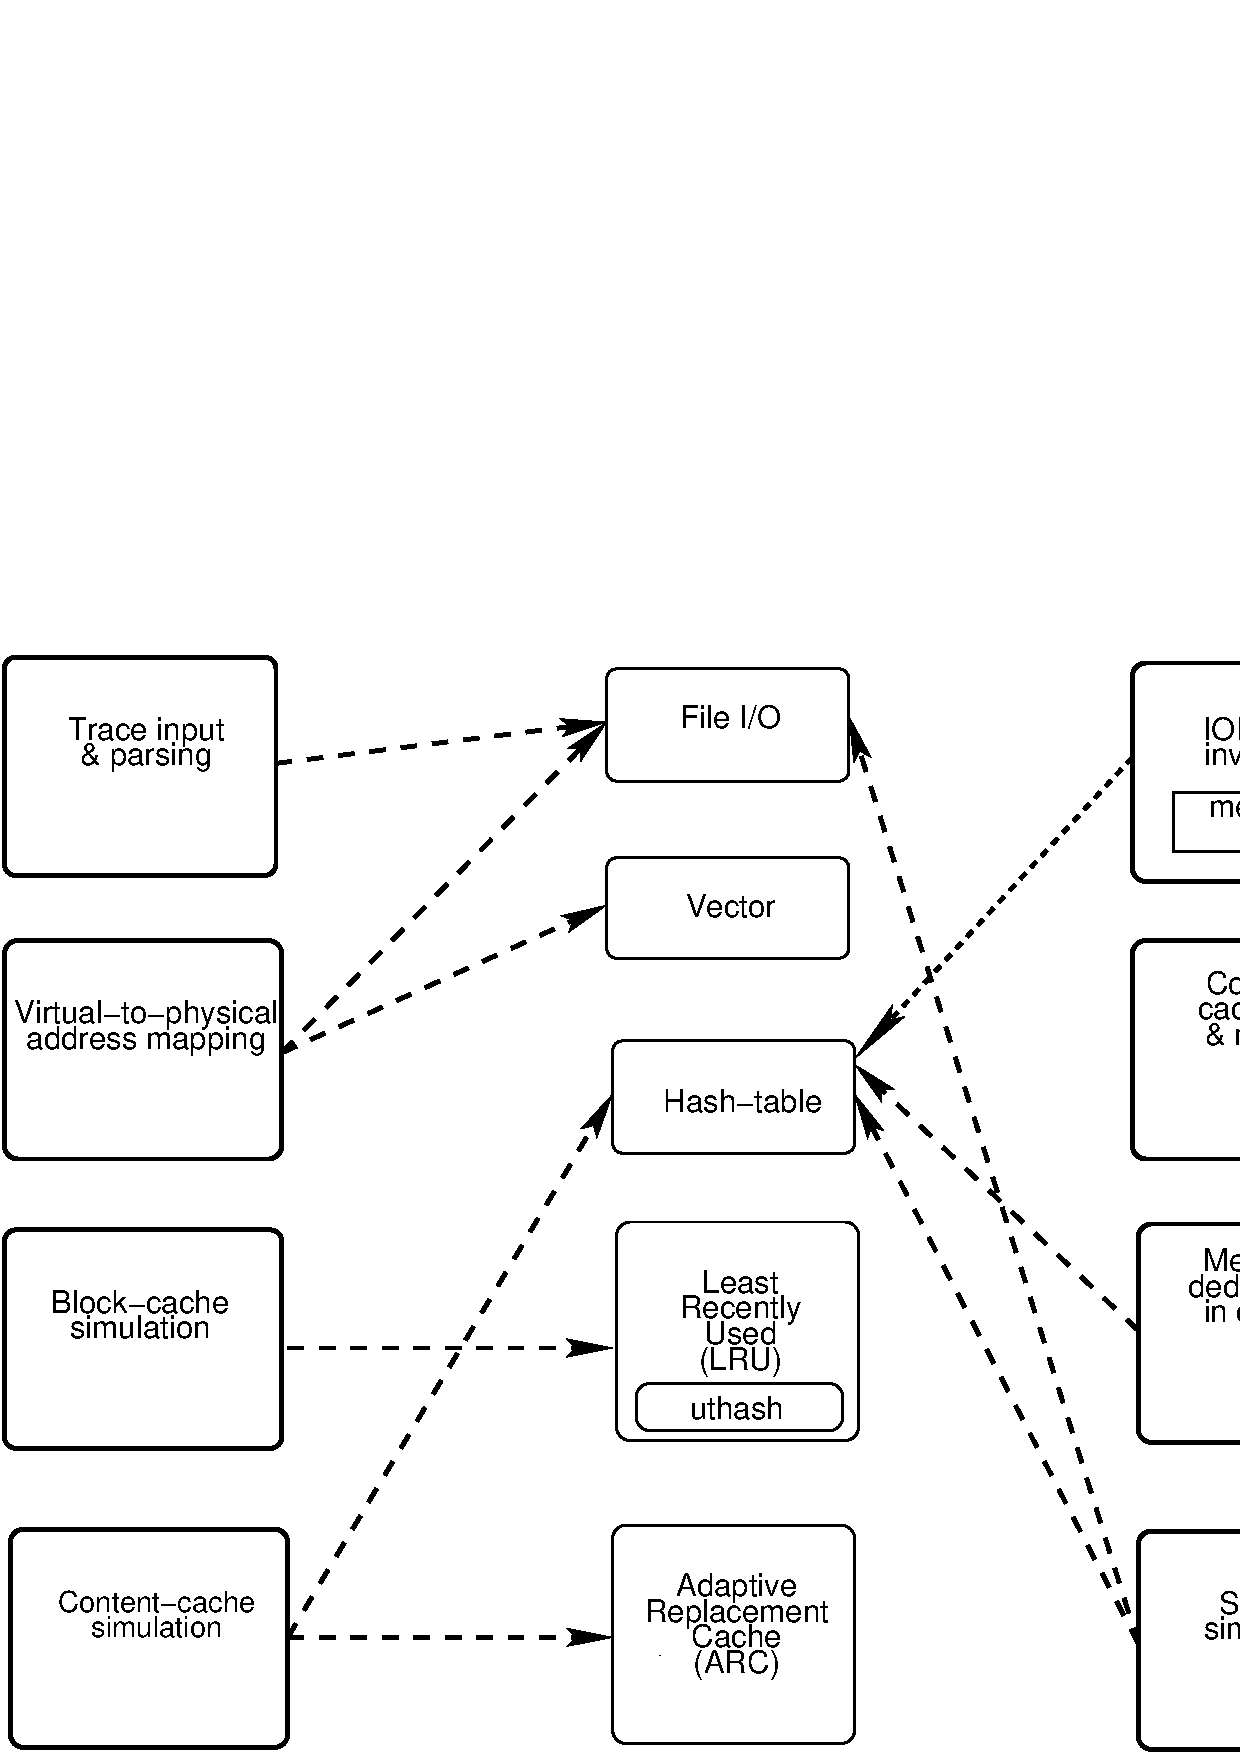
\includegraphics[scale=0.6]{simreplaychap-figures/simreplay-lowlevel.pdf}
%    \vspace{-0.1in}
    \caption{Low-level design of simulator: \textit{The left-most and the 
		right-most columns are the high-level components presented in 
		Fig.~\ref{fig:simreplay-interaction} and the center column contains
		the lower-level design components which underlie the
		higher-level design (as indicated by the unidirectional arrows).}}
    \label{fig:simreplay-lowlevel}
%    \vspace{-0.2in}
\end{figure}

Fig.~\ref{fig:simreplay-lowlevel} depicts the lower-level design for
each module specified in the earlier design diagram of 
Fig.~\ref{fig:simreplay-interaction}. In this section, we describe the
details of implementation of each of these modules in our simulator.

\subsection{Trace input \& parsing} 
\label{sec:simreplay-parsing}
%\subsection{Per-VM block requests}
%\paragraph{Input trace file format.} 
The trace files present at \cite{iodedup-online} has the following
format for every request:-
\begin{verbatim}
    [ts in ns] [pid] [process] [lba] [size in 512 Bytes blocks] [Write or 
	Read] [major device number] [minor device number] [MD5 per 4096 Bytes]
\end{verbatim}
The last column of the above format is in terms of the hexadecimal 
representation of the MD5 of the content. Hence, all above fields have
content in deterministic range, and parsing of the trace file can
be performed in a straight-forward line-by-line fashion. 

The above trace files represent a single workload each\textemdash{}\textit{webvm},
\textit{homes} or \textit{mail}, as mentioned earlier. However, our 
simulator is meant to simulate the replay of block requests of multiple
VMs on a single host. Hence, we accommodate an additional attribute, a VM
identifier, within each record in the trace. Accordingly, the 
data-structure representing a single request within the simulator is
as shown in Listing \ref{lst:vmreq}.

%\subsection{Parsing the input trace file}

\lstset{language=C,
	caption={Data-structure representing a single request.},
	label=lst:vmreq
}
\begin{snippet}
/* @vmname:  VM identifier
 * @time:    Time stamp when trace was emitted
 * @block:   VM I/O block identifier
 * @bytes:   Number of bytes transferred
 * @content: Content to be transferred
 * @rw:      Read (1) or write (0) 
 */
struct vmreq_spec {
    char vmname[HOSTNAME_LEN];
    __u64 time;
    __u32 block;
    __u32 bytes;
    __u8 *content;
    unsigned char rw:1;
};
\end{snippet}

\subsection{Addressing trace file inconsistencies by storage simulation}
\label{sec:simreplay-simdisk}
The trace files present at \cite{iodedup-online} have
the content (or rather, MD5 hash representation of content) along-with every read
and write request. This implies that a replay performed at a later
date can rely on these content for simulating storage reads and writes,
without having to actually perform the I/O on storage. However, our
experience with usage of these traces revealed that there were 
inconsistencies in the content reported in the traces. 

We define trace \textit{inconsistency} as the case where a piece of 
content was reportedly
read from or written to a block, but the next read request to the same
block reports another piece of content, although there were no writes to
that block in the interim. This could be caused due to some missing 
records in the trace. However, to evaluate the correctness of any 
replay module, the traces themselves would have to be consistent. Hence,
in our simulator, we maintain a simulated storage wherein the block
content is written to a file, and can be read back when required. In
this model, the first access to every block (whether read or write) is 
considered as the ground truth and written to the file (i.e. simulated 
storage). 
Naturally, subsequent write requests do not face any issues of consistency, 
since they are just new data to be written to storage.
However, for every subsequent read request, the content present on 
simulated storage is used for replay (since it is the consistent version), 
instead of
the content present in the trace (since it was found to be inconsistent 
at times).

\begin{figure}[t]
    \centering
    \includegraphics[scale=0.6]{simreplaychap-figures/simreplay-simdisk.pdf}
%    \vspace{-0.1in}
    \caption{Implementation of storage simulation in custom simulator. Each 
			hash-table entry contains an offset into the 
			\textit{simdisk} file.}
    \label{fig:simreplay-simdisk}
%    \vspace{-0.2in}
\end{figure}

The implementation of storage simulation in the custom simulator involves
usage of hash-tables and file I/O, as indicated in 
Fig.~\ref{fig:simreplay-lowlevel}. The file I/O module is required
because a file (referred as \textit{simdisk}) 
is used to store the content (or MD5 hash of content). 
Additionally, to enable ``storage-lookup'' using the block address,
we use a hash-table with the block address (string formatted) as the key.
Fig.~\ref{fig:simreplay-simdisk} presents a pictorial view of 
how storage simulation is implemented in our simulator.
Within the hash-table entry that is identified for a given block, we 
maintain a file offset value which indicates the offset within the 
\textit{simdisk} file, at which the corresponding content is stored.

\subsection{Mapping from virtual disk space to physical disk space}
As mentioned in Section~\ref{sec:simreplaychap-v2p},
the input V2P mapping
indicates the range of physical blocks (i.e. blocks on host storage)
that map to the address space of each VM (i.e. blocks of virtual disk)
for simulation. 
For a trace replay file that has a single VM's requests, 
this input file is not mandatory, since the simulator can infer this map
dynamically from the trace file itself. 
In fact, at the end of the 
simulator invocation, the inferred V2P map is output to the same
file. Thus, with a single-VM trace file, it is possible to determine
the range of blocks (i.e. maximum block number accessed) for that VM.
However, in case of a trace input
file that has aggregated requests from multiple VMs, this input file is 
mandatory and it is validated that the ranges of blocks specified for 
each VM does not overlap with the range of any other VM. 
In order to
build this multi-VM input V2P file, the output V2P file(s) from the single-VM
trace executions can be used additively, as indicated in 
Section \ref{sec:simreplaychap-v2p}.

The input of V2P mapping requires the file 
I/O module (refer Fig. \ref{fig:simreplay-lowlevel}) since the mapping
has to be read from and written to a file. Also, after receiving the 
input mapping, the simulator uses a vector data-structure for storing
the 3-tuples for each VM involved in replay.
The \textit{vector} data-structure is basically the same as an array, 
except that it can grow as required, unlike an array which has static
size allocation.

%\subsection{Enabling input of mapping}
%A file can be specified using option -m which should contain a 3-tuple of
%above format per line. Each line is for one VM. 
%\subsection{Implementation}
%Using vectors to store a 3-tuple consisting of \textit{vmname},
%base block address per VM, and capacity per VM.

\subsection{Block-cache simulation}
%\subsection{Implementation details}
Since the block-cache needs to be looked-up by block ID, a hash-table
implementation is required. Also, since the LRU policy has to be applied
to the elements in the block-cache, all such elements should also form
part of a linked list. Instead of implementing this cache from scratch,
we used an existing hash-table implementation called 
\texttt{uthash}\cite{uthash}, which is basically a hash-table for 
storing C data-structures. It requires that a \textit{UT\_hash\_handle}
element be added to the data-structure that is to be stored into the
hash-table and another field (say blockID) of the same data-structure 
can be used as the key to lookup the hash-table. 

The \texttt{uthash}
module also maintains a linked list of all the elements in the hash-table
in ``insertion'' order. In order to simulate LRU policy for the
block-cache, we have to tweak the ordering slightly, as follows.
If a block is already present in the hash-table, inserting it again
for the same key is an error in the \texttt{uthash} module. Modifying it 
in-place is not an error though, but it will not cause the LRU ordering
that we require. So, when we find that the block being requested is in cache,
we first delete it from the hash-table, and then re-insert it,
to simulate LRU ordering.

\subsection{IODEDUP metadata store}
In our simulator, we have designed and implemented the IODEDUP metadata
store in a similar fashion as the DRIVE metadata store except for two 
major differences: (i)~The DRIVE metadata store is present within the
virtual address space whereas the IODEDUP metadata store holds mapping
within the physical storage address space, (ii)~The DRIVE metadata store
maintains implicit caching hints to aid in request redirection whereas IODEDUP
metadata store is used to retrieve the content hash which is further used
for content-cache lookup.

\subsection{Content-cache simulation}
The content-cache is implemented using a hash-table implementation,
and has the Adaptive Replacement Cache (ARC) as the cache replacement
policy. The ARC policy basically maintains four lists\textemdash{}(i) a list of
in-cache elements in the LRU order, (ii)~a list of in-cache elements
in the LFU order, (iii)~a list of recently-evicted (ghost) elements 
in the LRU order, and (iv)~a list of ghost elements in the LFU order.
The ARC algorithm uses these four lists and maintains their relative
sizes in order to most effectively keep the most recently used and
the most frequently used elements in cache. 

In our implementation, we use an online implementation of the ARC
algorithm for the content-cache simulation. The content-cache can
be looked up based on the hash of the content, and the insertion/deletion
in cache is performed according to ARC policy mentioned above.
For a read request, the content-cache needs to be looked up only
upon a metadata hit in the IODEDUP system. In case of a metadata
miss, the read request is forwarded to the storage instead.
For a write request, the content-cache is written into and the
metadata is updated accordingly. The content-cache is maintained
with write-through semantics, as specified in~\cite{iodedup}.

\subsection{Quantifying content-deduplication in cache(s)}
The aim of this simulator is to study cache management effectiveness,
and we quantify the content deduplication effected within the cache(s) 
(including the content-cache as well, for IODEDUP)
as a measure of its effectiveness. In our simulator, we simulate 
traps at every block insertion and eviction from cache(s).
A separate hash-table is maintained which keeps track of the duplicate
content among the blocks currently present in the simulated cache(s), 
and this hash-table is modified at every such interrupt/trap occurrence.

In case of a block being inserted into the cache, in the trap
that ensues, we fingerprint it 
and lookup the hash-table to see if there are any other blocks already
in cache(s) with the same fingerprint. If so, its reference counter is
incremented. When a block is evicted from cache, the trap processing
again involves fingerprinting it and searching the hash-table. If
the content is present in the hash-table, its reference counter is 
decremented, and the entry is removed from the hash-table if the 
reference counter reaches value of zero.
At any instance during replay, the \textit{content deduplication factor}
can be defined as the ratio of number of unique blocks in cache(s) to 
number of total blocks in cache(s). Higher the content deduplication
factor, higher the efficiency of the cache space utilization, and hence
higher the storage access performance.


\subsection{Verifying the correctness of the simulator}
To ensure correctness of the simulator, each individual module was
first unit-tested manually with small input sizes, and then the entire
module as a whole was integration-tested with whole trace files. 
For every block that is present in cache (whether block-cache 
or content-cache), it is verified that the content present on the 
simulated storage is actually the same as the content returned from
cache. Note that this is only a simulation-correctness check and does not 
count towards number of disk reads for replay.
Additionally, for each invocation of the simulator, the following are 
verified in code (using assert statements).
\begin{itemize}
\item The total number of \textit{reads} replayed equals the sum of 
\textit{cache hits} and \textit{cache misses}.
\item The total number of \textit{cache hits} equals the sum of 
\textit{read cache hits} and \textit{write cache hits}.
\item The number of \textit{read cache misses} equals the number
of \textit{disk reads}.
\item The number of \textit{read cache misses} equals the sum of
\textit{compulsory} and \textit{capacity misses}.
\item The total number of \textit{writes} replayed equals the total number
of blocks written to disk.
\end{itemize}


\section{Input options and usage}
\label{sec:simreplaychap-usage}

Listing \ref{lst:usage} shows the basic usage options for the custom
simulator, \textit{simreplay}, in alphabetic order. Each option is
explained below.

\lstset{language=C,
	caption={Listing of simreplay usage},
	label=lst:usage
}
\begin{snippet}
static char usage_str[] =                                               \
        "\n"                                                            \   
        "\t[ -C        : --iodedup-logformat        ] Default: 0\n"     \   
        "\t[ -d <dir>  : --input-directory=<dir>    ] Default: .\n"     \   
        "\t[ -e        : --read-enable              ] Default: Off\n"   \   
        "\t[ -E        : --write-enable             ] Default: Off\n"   \   
        "\t[ -f <file> : --input-file=<file>        ] Default: None\n"  \   
        "\t[ -h        : --help                     ] Default: Off\n"   \   
        "\t[ -m <file> : --mapv2p=<file>            ] Default: None\n"  \   
        "\t[ -O <in-MB>: --overall-RAM-size=<in-MB> ] Default: 1024\n"  \   
        "\t[ -o <in-MB>: --contentcache-size=<in-MB>] Default: 100\n"   \   
        "\t[ -Q        : --Vanilla-replay           ] Default: On\n"    \   
        "\t[ -R        : --DRIVE-replay             ] Default: Off\n"   \   
        "\t[ -T        : --IODEDUP-replay           ] Default: Off\n"   \   
        "\t[ -V        : --version                  ] Default: Off\n"   \   
        "\n";	
\end{snippet}

The option \texttt{iodedup-logformat} indicates that the content information
present in each trace request is in terms of the MD5 hash of the content,
as is the case with the traces \textit{webvm}, \textit{homes} and
\textit{mail} available online at \cite{iodedup-online}. 
This flag is especially useful for parsing of the input trace file.
When the flag is specified, the content field is expected to be 32 
characters (i.e hexadecimal representation of 16-byte MD5 hash). On the 
other hand, if this flag is 
not specified, the original content is expected to be present in the trace. 
For example, if \texttt{iodedup-logformat} is not indicated, the size of the 
content is equal to the value in the \texttt{nbytes} field in the trace
request data-structure.

The options \texttt{input-directory} and \texttt{input-file} are used
to specify the input trace file to be used for simulated I/O replay. The
file contains multiple read/write requests, each in the format described
earlier. Parsing of the file is performed by the "Trace input \& parsing
module" as discussed in Section \ref{sec:simreplay-parsing}.

The options \texttt{read-enable} and \texttt{write-enable} indicate whether
read requests or write requests should be replayed, respectively. If 
\texttt{read-enable} is not specified, read requests replay will not be 
simulated and if \texttt{write-enable} is not specified, write requests 
will not be simulated. Note that, at least one of these two options 
has to be specified otherwise there is no simulation to be done.
By default, both options are disabled, however a typical invocation of
simulator would enable both options so that all read and
write requests present in the trace file would be replayed/simulated.

The option \texttt{mapv2p} can be used to specify the input V2P mapping
indicating the range of physical blocks that map to the address space of 
each VM, as described earlier.
If the trace file has only a single VM's requests, the input V2P
mapping is optional, but is mandatory otherwise.

The option \texttt{overall-RAM-size} indicates the space in 
number of megabytes (MB) to be simulated as the block-cache in the
Vanilla system. By default, the value is 1024 MB, i.e. 1GB block-cache.
This option is also applicable to the IODEDUP system, but in conjunction
with the value specified using the option \texttt{contentcache-size},
as follows. The option \texttt{contentcache-size} specifies what portion
of the \texttt{overall-RAM-size} should be simulated as a content-cache,
and defaults to 100 MB.
This option is valid only for IODEDUP replay, and re-adjusts the configured
size of the block-cache to \texttt{overall-RAM-size} minus 
\texttt{contentcache-size}. It follows that, the value of 
\texttt{contentcache-size} must be less than or equal to 
\texttt{overall-RAM-size}, for successful invocation of the simulator.

\lstset{language=bash,
	caption={Sample output of \texttt{SimReplay} for Vanilla invocation.},
	label=lst:vanilla-sample
}
%\begin{minipage}[t][5cm][b]{0,5\textwidth}
%\begin{Verbatim}[frame=single]
\begin{snippet}
$ cat stats-O1024-webvm-iodedup-sreplay_rw.txt
#READ=3116456, #WRITE=11177702
RAM-size = 1024 (MB)
buffer cache: hits=12303451, misses=1990707, readhits=1471112, writehits=10832339
disk hits=12823046
disk hits read=1645344, writes=11177702
\end{snippet}
%\end{Verbatim}
%\end{minipage}

\lstset{language=bash,
	caption={Sample output of \texttt{SimReplay} for IODEDUP invocation.},
	label=lst:iodedup-sample
}
\begin{snippet}
$ cat stats-O1024-o100-webvm-iodedup-ioreplay_rw.txt 
io-redirections: self-is-leader=813572, self-is-not-leader=1409885
read-responses: compulsory-misses=316045, cache-hits=704111, capacity-misses=2096300
metadata-hit-conversions: deduphits=127156, selfhits=1, dedupmisses=1282729, selfmisses=813571
#READ=3116456, #WRITE=11177702
RAM-size = 1024 (MB)
CCACHE-size = 100 (MB)
buffer cache: hits=11185632, misses=3108526, readhits=576954, writehits=10608678
content metadata: hits=2223457, misses=316045 dirties=0
content cache: hits=127157, misses=8035550
content cache: dedup hits=127156, nondedup hits=1
disk hits=13590047
disk hits read=2412345, writes=11177702
\end{snippet}

\lstset{language=bash,
    caption={Sample output of \texttt{SimReplay} for DRIVE invocation.},
    label=lst:drive-sample
}
\begin{snippet}
cat stats-O1024-webvm-iodedup-freplay_rw.txt 
io-redirections: self-is-leader=1754745, self-is-not-leader=1045666
read-responses: compulsory-misses=316045, cache-hits=2722411, capacity-misses=78000
metadata-hit-conversions: deduphits=1033328, selfhits=1689083, dedupmisses=12338, selfmisses=65662
#READ=3116456, #WRITE=11177702
RAM-size = 1024 (MB)
confided metadata: hits=2800411, misses=316045, mapmisscachehits=0, dirties=0, mapdirtycachehits=0
fcollisions=0, fcollisionstp=3141002, fzeros=0
buffer cache: hits=13635026, misses=659132, readhits=2722411, writehits=10912615
disk hits=11571747
disk hits read=394045, writes=11177702
\end{snippet}

The options \texttt{Vanilla-replay} and \texttt{IODEDUP-replay} indicate
that the simulator is to be invoked to simulate Vanilla execution and
IODEDUP execution, respectively.
Listings \ref{lst:vanilla-sample} and \ref{lst:iodedup-sample} 
show sample outputs of the simulator when used for Vanilla and
IODEDUP invocations, respectively.
Similarly, the option \texttt{DRIVE-replay} indicates that the
simulator is to be invoked to simulate DRIVE execution.
A sample output of DRIVE invocation of the simulator 
is shown in Listing~\ref{lst:drive-sample}.

The sample output of Vanilla invocation in Listing~\ref{lst:vanilla-sample}
has information regarding the number of read and write requests in the trace,
the total cache (RAM) size used, the number of hits and misses in the 
buffer (block) cache, and a classification of the hits into reads hits or
write hits as well. Finally, it also reports the number of requests that
went to disk\textemdash{}in case of reads, this is the number of disk 
reads that happened, and in case of writes, this is the total number of
writes since we assume that all writes are flushed to disk eventually.

The sample output of IODEDUP and DRIVE invocation also have similar fields
as above, however they have some additional fields too, to track the
efficiency achieved by each system. For example, Listing \ref{lst:iodedup-sample}
presents information regarding the configured size of content-cache,
the number of metadata hits incurred, and how many of those were for
reads and writes, each. It also presents information regarding how many
of the metadata hits eventually resulting in content-cache hits and misses.
Additionally, for all of the content-cache hits, it lists how many were hits for
duplicate content and how many were just regular hits.

The \texttt{help} option shows the usage listing 
for the \texttt{SimReplay} tool, and the
\texttt{version} option can be used to identify different versions of
the custom simulator, for future extension.

